\documentclass[]{article}
\usepackage[utf8]{inputenc}
\usepackage{fullpage,ifpdf,url,authblk,xspace}
\usepackage{url}

\renewcommand\Affilfont{\small}

\ifpdf
\usepackage[pdftex]{graphicx}
\else
\usepackage{graphicx}
\fi


\title{Simple, Current, Recommendations Based on Activity-based User Profiles}

\author[1]{Libby Miller}
\author[2]{Dan Brickley}
\author[1]{Vicky Buser}
\author[1]{Yves Raimond}
\author[3]{Members of the NoTube project}

\affil[1]{BBC, UK}
\affil[2]{Vrije Universiteit, Amsterdam}
\affil[3]{http://notube.tv}


\begin{document}


\ifpdf
\DeclareGraphicsExtensions{.pdf, .jpg, .tif}
\else
\DeclareGraphicsExtensions{.eps, .jpg}
\fi

\maketitle

\abstract{In the NoTube project we have used BBC linked data to prototype a profile-based simple recommender service: below we describe the details of the implementation, including profile generation, the recommendations produced, the role of BBC programmes data, and further work.}

\section{The Goal}

Our goal is to demonstrate an end-to-end implementation of a simple recommender based on a user profile derived from their online social activity. To limit scope, in the first instance we use one social network and BBC data only. In this part of the project we are looking primarily at broadcast data so the focus is on recommendations for the current day. In parallel, within the NoTube project, work is going on to enrich non-BBC programmes data to produce useful recommendations in the more general case. This is discussed elsewhere.

\section{BBC Linked Data}

The BBC aims to publish an RDF page along side the HTML page for each programme it produces. These contain data about the programme, its brand, series, when it was broadcast, and on which service, its contributors, genres and other linked information. In some cases there are links to DBPedia URLs and MusicBrainz URLs, but the majority of the data uses BBC links, and is described in the BBC Programmes Ontology\footnote{\url{http://www.bbc.co.uk/ontologies/programmes/}}.

This is a very useful dataset for prototyping recommendations as (a) it's all in RDF and (b) SPARQL stores are available to access it (c) it is fairly rich and well-connected, without having to add to it, and (d) all channels, programmes (and brands, series etc) have unique URLs following linked data principles and based on 8-15 alphanumeric character programme ids (PIDs).

\section{Profile Generation}

The Beancounter profile generator\footnote{\url{http://data.semanticweb.org/workshop/sdow/2009/paper/1/html}} can already generate profiles based on DPPedia, but for the purposes of this demonstrator we wanted to gather data specifically about BBC PIDs, which are mentioned on Twitter in sufficient numbers to be useful. We implemented a simple Twitter-based profiler that takes the last two hundred public tweets for a given user, parses out BBC programme identifiers, gathers information about the programmes from a SPARQL datastore of BBC programmes, and summarises the result with a simple counter. This is just temporary until Twitter and BBC data enhancement are fully implemented in the Beancounter.

Here are the steps:
\begin{itemize}
\item{Retrieve ten pages of data for (say) libbymiller using the twitter API}
\item{Use a regex to parse out the 8 digit PIDs}
\item{Do the following SPARQL query over the programmes data store, which gets categories, contributors, brands, series:}
\end{itemize}

\begin{verbatim}
PREFIX po: <http://purl.org/ontology/po/>
SELECT ?result
WHERE {
{<http://www.bbc.co.uk/programmes/#{pid}#programme> po:masterbrand ?result .} UNION
{<http://www.bbc.co.uk/programmes/#{pid}#programme> po:category ?result . } UNION
{?result po:episode <http://www.bbc.co.uk/programmes/#{pid}#programme> . }
}
\end{verbatim}


\begin{itemize}
\item{Counts the number of each distinct ?result}
\item{Looks up their type and label}
\item{Outputs the result as RDF and HTML - see Fig \ref{htmlprofile} for the HTML version}
\end{itemize}

\begin{verbatim}
<foaf:Person>
...
<wi:preference>
  <wi:WeightedInterest>
    <wi:topic rdf:resource="http://www.bbc.co.uk/services/radio4#service" />
    <rdf:type rdf:resource="http://purl.org/ontology/po/Service"/>
    <rdfs:label>BBC Radio 4</rdfs:label>
    <wi:weight>5</wi:weight>
    <wi:scale>0..26</wi:scale>
    <wi:context rdf:resource="#default" />
  </wi:WeightedInterest>
</wi:preference>
<wi:preference>
  <wi:WeightedInterest>
    <wi:topic rdf:resource="http://www.bbc.co.uk/programmes/places/VGVmL2xvY2F0aW9uL2dlbmV2YQ#place" />
    <rdf:type rdf:resource="http://purl.org/ontology/po/Category"/>
    <rdfs:label>geneva</rdfs:label>
    <wi:weight>1</wi:weight>
    <wi:scale>0..26</wi:scale>
    <wi:context rdf:resource="#default" />
  </wi:WeightedInterest>
</wi:preference>
</foaf:Person>
<wi:Context rdf:about="#default">
<wi:timePeriod>
 <days:DayInterval> <!-- i.e. every day, all day -->
  <tl:at rdf:datatype="http://www.w3.org/2001/XMLSchema#time">00:00:00</tl:at>
  <tl:end rdf:datatype="http://www.w3.org/2001/XMLSchema#time">23:59:59</tl:end>
 </days:DayInterval>
</wi:timePeriod>
</wi:Context>
\end{verbatim}

\begin{figure}[h] 
\begin{center}
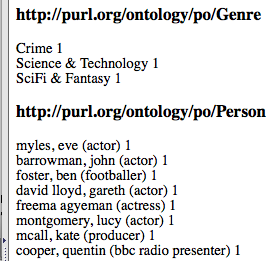
\includegraphics[width=6 cm]{htmlprofile.png}
\caption{Simple HTML profiles}
\label{htmlprofile}
\end{center}
\end{figure}


\section{Recommendation}

These recommendations are really just a way to filter what is on TV on a given day with respect to a profile, so the technique is very simple.\footnote{There is other more sophisticated work going on for recommendations in the linked data area - see for example \url{http://dbrec.net/} and \url{http://github.com/moustaki/rqommend}}. The basic process is:

\begin{itemize}
\item{Retrieve the user's weighted interest profile}
\item{Get the data, ordering by weight}
\end{itemize}

\begin{verbatim}
PREFIX wi: <http://xmlns.notu.be/wi#>
PREFIX rdfs: <http://www.w3.org/2000/01/rdf-schema#>
SELECT DISTINCT ?url ?label ?weight ?scale
where {
  ?thing wi:topic ?url .
  ?thing rdfs:label ?label .
  ?thing wi:weight ?weight .
  ?thing wi:scale ?scale .
}
ORDER BY ?name DESC(?weight)
\end{verbatim}

\begin{itemize}
\item{For each url (genre, brand etc) in order of weight, look for matches that are on today}
\item{Look up time, channel, title, description and brand}
\item{Generate a reason for the recommendation (e.g. `you watched this series 10 times')}
\item{Output the channel, datetime, title, description and reason for recommendation in the appropriate format}
\end{itemize}

\begin{figure}[h] 
\begin{center}
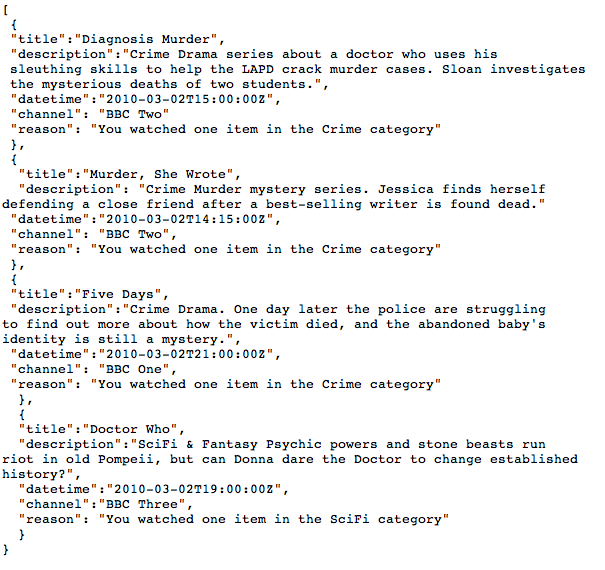
\includegraphics[width=12 cm]{basicrecommendations.png}
\caption{Basic Recommendations}
\label{basicrecomendations}
\end{center}
\end{figure}


\section{MythTV}

MythTV uses a series of XML templates to display information onscreen, such as the programme guide (EPG). It has a categorisation feature which can show programmes with different categories in different colours in the EPG. For this demonstration, we simply created a new recommendations category in the template with a new colour, and supressed the other categories. We then injected the category recommendations into the appropriate field for the recommended programmes in the underlying MythTV database.

\begin{figure}[h] 
\begin{center}
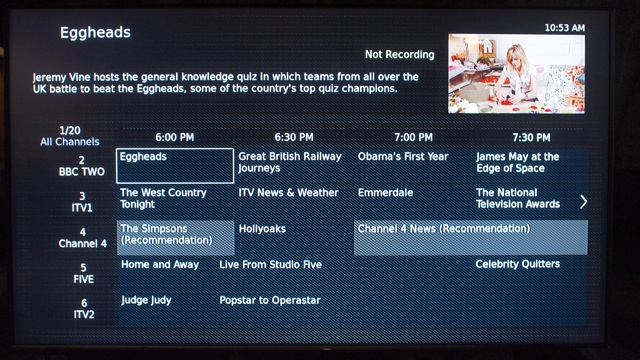
\includegraphics[width=12 cm]{mythtv-recommendations.jpg}
\caption{Basic Recommendations in MythTV UI}
\label{mythrecs}
\end{center}
\end{figure}

\section{Implementation}

The profile generator is written using a simple Ruby servlet with a specific class to make SPARQL access to 4Store simple.\footnote{http://github.com/moustaki/4store-ruby}. The recommender uses Jruby and Jena TDB in order to store and query the profile data. The MythTV data injection used a ruby script on a crontab.

\section{Future Work}

This is a very basic prototype and there is a great deal of work to be done. Here are some issues we found with this implementation.

\subsection{Quality of the Recommendations}

The recommendations were reasonably good, but they were also rather conventional. It is unlikely anyone would try watching anything very new following these. More interesting links between items (e.g. from DBPedia) would help here, as would more variety of input  to the profile (e.g. random inclusions, adding friends' data).

\subsection{Contexts in Profiles}

The recommendations are based on the entire days' programming; contextual information (for example about what is preferred by the user at a particular time of day) might help improve them.

\subsection{Finding Data}

Most people do not, of course, commonly use BBC programmes URLs when talking about programmes on Twitter or elsewhere, either because they cannot copy and paste, are not online, do not know about the URLs or do not care. Non-BBC programmes do not generally have unique identifiers in any case. We need to investigate heuristics for finding programmes mentioned in this way, or focus our attention on activity streams that do output useful data.

\subsection{Using non-BBC data}

Work is underway to provide an enriched database of BBC and non-BBC data using various enhancement tools, including entity recognition from DBPedia and elsewhere, `same-as' services and lookup services.

\subsection{Architectural issues}

Enhanced profile generation can take a long time, so there is a need for a callback feature that can remind the user (or application) to return. This is being addressed in the Beancounter.

Currently the location of the profile generator and the recommender are hardcoded into the set top box and run off a crontab, while usernames and passwords are passed from a control device.\footnote{We will write a separate paper on our work with jabber, MythTV and the iPhone}.  In our model, the user's identity is held in the control device, not the set top box, so because recommendations can also take a while to generate, it will take a while for recommendations to become available if they are only triggered when the user indicates on the control device that she wants to watch TV.

It may therefore make sense for to create a web-based user interface which can be used both to access the Beancounter and to trigger recommendations from a given profile, without the recommender being too highly integrated with the Beancounter.

\subsection{RDF Tool Availability}

Ruby was chosen as development language because it is extremely quick to prototype with; however RDF tool support is poor in it. Jruby and Jena provided a good solution to this however.

\end{document}
